\part{Implémentation}

\chapter{Implémentation}
Vous trouverez également ci-joint une courte vidéo montrant notre application en action.

\section{Copies d'écran de l'implémentation}
Ci-dessous quelques impressions de l'implémentation :

\begin{center}
	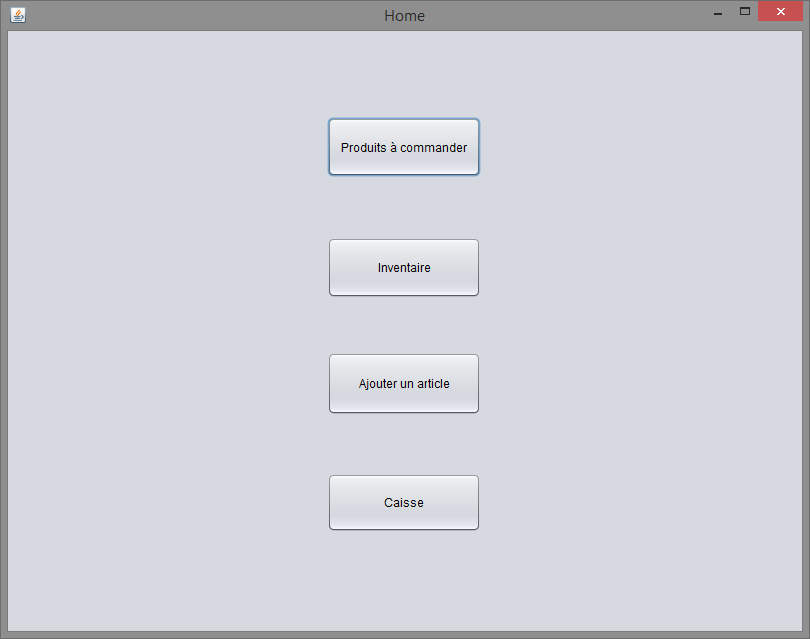
\includegraphics[width=14cm]{./Implementation/home}
\end{center}

\begin{center}
	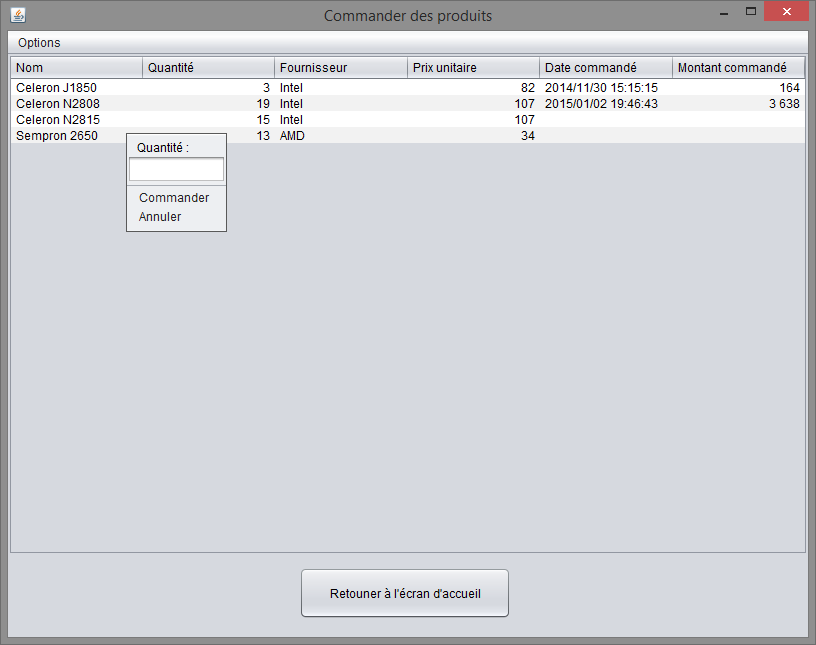
\includegraphics[width=14cm]{./Implementation/acommander}
\end{center}

\begin{center}
	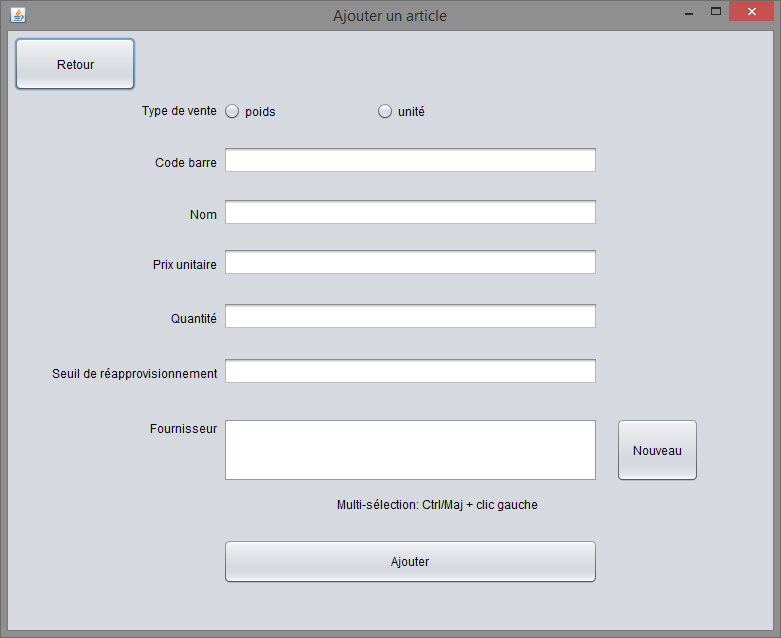
\includegraphics[width=14cm]{./Implementation/ajouteraticle}
\end{center}

\begin{center}
	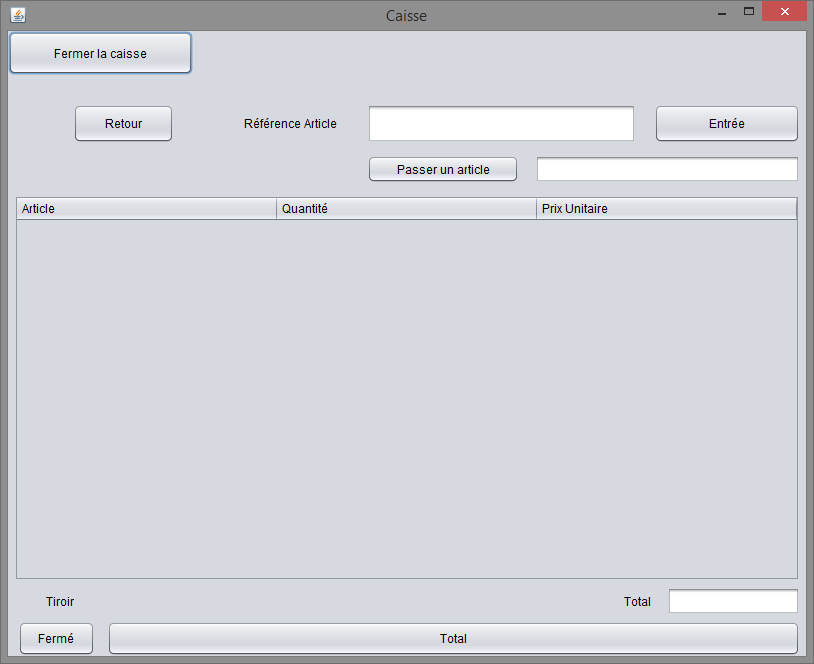
\includegraphics[width=14cm]{./Implementation/caisse}
\end{center}

\begin{center}
	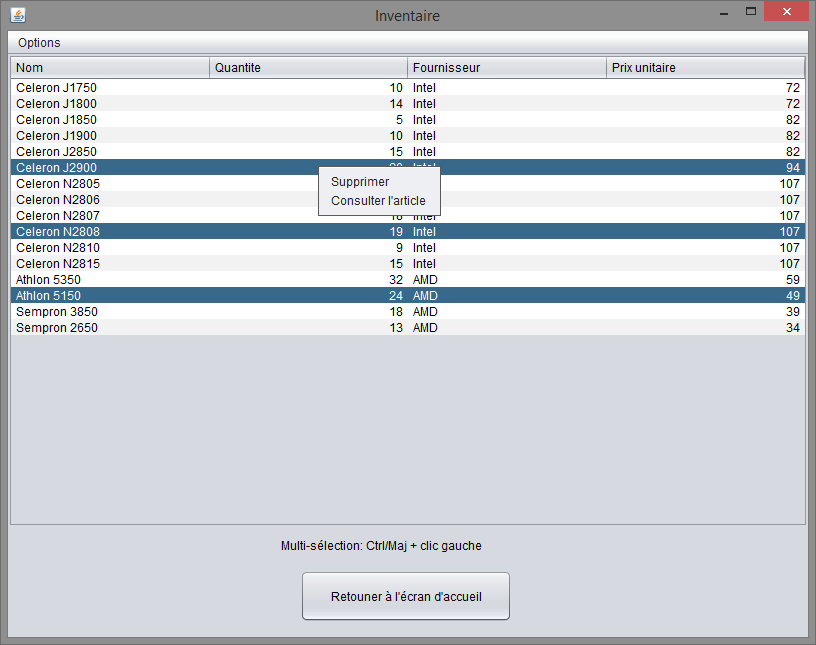
\includegraphics[width=14cm]{./Implementation/inventaire}
\end{center}

\begin{center}
	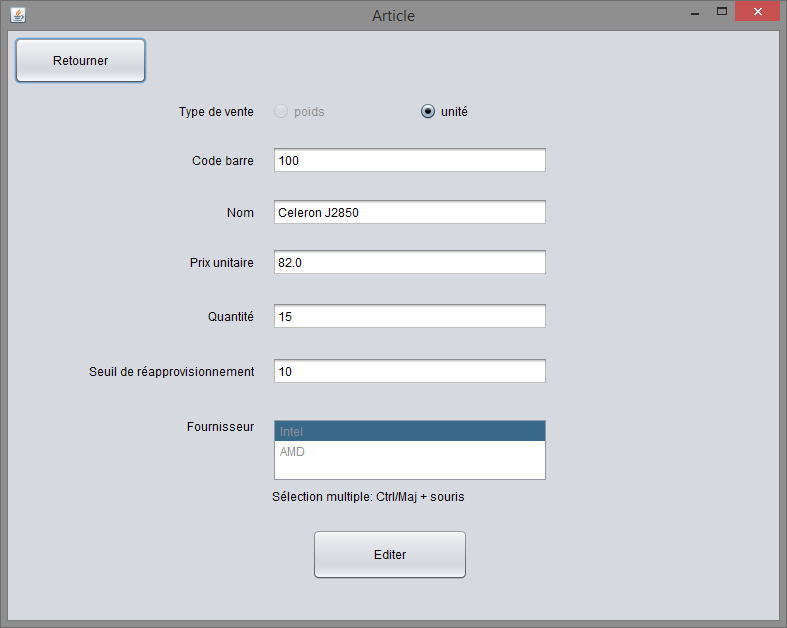
\includegraphics[width=14cm]{./Implementation/article}
\end{center}

\section{Livrable du logiciel}

\subsection{Installation}
\begin{enumerate}
	\item Ouvrez le projet avec Netbeans.
	\item Dans l'onglet \textit{Service}, créez une nouvelle base de donnée nommé \textbf{uml} avec en identifiant : \textbf{uml} et en mot de passe : \textbf{groupe3}. 
	\item Connectez vous à cette nouvelle base de donnée.
	\item Faites un click droit sur la base de donnée et sélectionnez \textit{exécuter}.
	\item Copiez-collez le script scriptBDD.sql et exécutez le script
	\item Copiez-collez le script ajoutBDD.sql et exécutez le script
	\item Vous pouvez maintenant lancer notre application
\end{enumerate}

\subsection{Mode d'emploi}
Une fois le programme lancé, suivez simplement les indications sur l'écran et naviguez à l'aide des boutons.

\section{Bilan de l'état du projet}
Notre solution remplit auourd'hui toutes les exigences du cahier des charges. Cependant il est envisageable d'imaginer d'autres possibilités. 

Il serait ainsi intéressant de garder en mémoire les articles passés en manuel à la caisse pour, dans le cas échéants, corriger le code barre.

Le cahier des charges ne le précise pas, mais la possibilité de passer commande de plusieurs articles dans une même commande pourrait être ajoutée. 

Une grosse évolution serait la mise en place d'une API côté serveur. Ainsi des clients, type mobile, pourraient vérifier l'état des stocks n'importe où et n'importe quand. 